\section{Tamtam Listens}
\label{sec:tamtam-listens}

La aplicación desarrollada, denominada \emph{Tamtam Listens}, es el resultado de la combinación
de las tecnolog\'ias mencionadas anteriormente. Por lo tanto, \emph{Tamtam Listens} representa una
interfaz de interacci\'on alternativa para la aplicaci\'on \emph{Tamtam Edit}.

El reconocimiento de los comandos de voz se implement\'o como un servicio de \emph{dbus}\cite{Dbus2013}, que es
un mecanismo para comunicaci\'on entre procesos de linux. Por lo tanto, el servicio puede ser utilizado
no solo por \emph{Tamtam Listens} si no por cualquier aplicaci\'on de linux. 

\emph{Pocketsphinx} requiere de un modelo ac\'ustico y un modelo de lenguaje para realizar
el reconocimiento de comandos. Para el modelo ac\'ustico se utiliz\'o el prove\'ido por el proyecto \emph{Voxforge}
\cite{Voxforge}, que es un proyecto que busca proveer modelos ac\'usticos para motores de reconocimientos
de c\'odigo abierto. Para el modelo de lenguaje se defini\'o una gram\'atica JSGF\cite{JSGF2000}, que permiti\'o definir los
comandos soportados por la aplicaci\'on de una manera sencilla. 

\subsection{Gram\'atica}

A continuaci\'on se puede observar un fragmento de la gram\'atica JSGF utilizada para definir 
los comandos soportados por \emph{Tamtam Listens}, m\'as adelante se presentar\'an los comandos
en forma de grafo para una mejor comprensi\'on.

\lstset{
  basicstyle=\scriptsize,        % the size of the fonts that are used for the code
  breakatwhitespace=false,         % sets if automatic breaks should only happen at whitespace
  frame=single,                    % adds a frame around the code
  language=Octave,                 % the language of the code
  numbersep=5pt,                   % how far the line-numbers are from the code
  showstringspaces=false,          % underline spaces within strings only
  stepnumber=2,                    % the step between two line-numbers. If it's 1, each line will be numbered
  tabsize=2                       % sets default tabsize to 2 spaces
}

\begin{figure}[H]
\begin{lstlisting}
#JSGF V1.0;
grammar tamtam;

public <tamtam-listens> = <comando> | <pagina> | <pista-a>     | <pista-b>  | 
                          <seleccionar-compas> | <crear-nota>  | <seleccionar-nota> | 
                          <duplicar-nota>      | <borrar-nota> | <volumen> | <tempo> | 
                          <configurar-nota>    | <loop>;

<comando>  = REPRODUCIR MUSICA  | PAUSAR MUSICA   | PARAR MUSICA | GENERAR MUSICA | 
             CREAR NUEVA MUSICA | EXPORTAR MUSICA | SALIR DE TAMTAM;
<pagina>   = ( CREAR NUEVA | DUPLICAR | LIMPIAR ) PARTITURA | PARTITURA <orden>;
<orden>    = ( ANTERIOR | SIGUIENTE );
<loop>     = (BASURA)+;
\end{lstlisting}
\caption{Fragmento de la gram\'atica utilizada en \emph{Tamtam Listens}}
\end{figure}

Los comandos pueden clasificarse en Generales (G), de Pista (P) y de Comp\'as (C). A continuaci\'on
se presentan los distintos comandos soportados, utilizando grafos para representarlos y as\'i facilitar
su comprensi\'on. El nodo coloreado hace referencia a la \'ultima palabra de un comando v\'alido para la aplicaci\'on

\subsubsection{Comandos Generales}

\begin{figure}[H] 
\centering
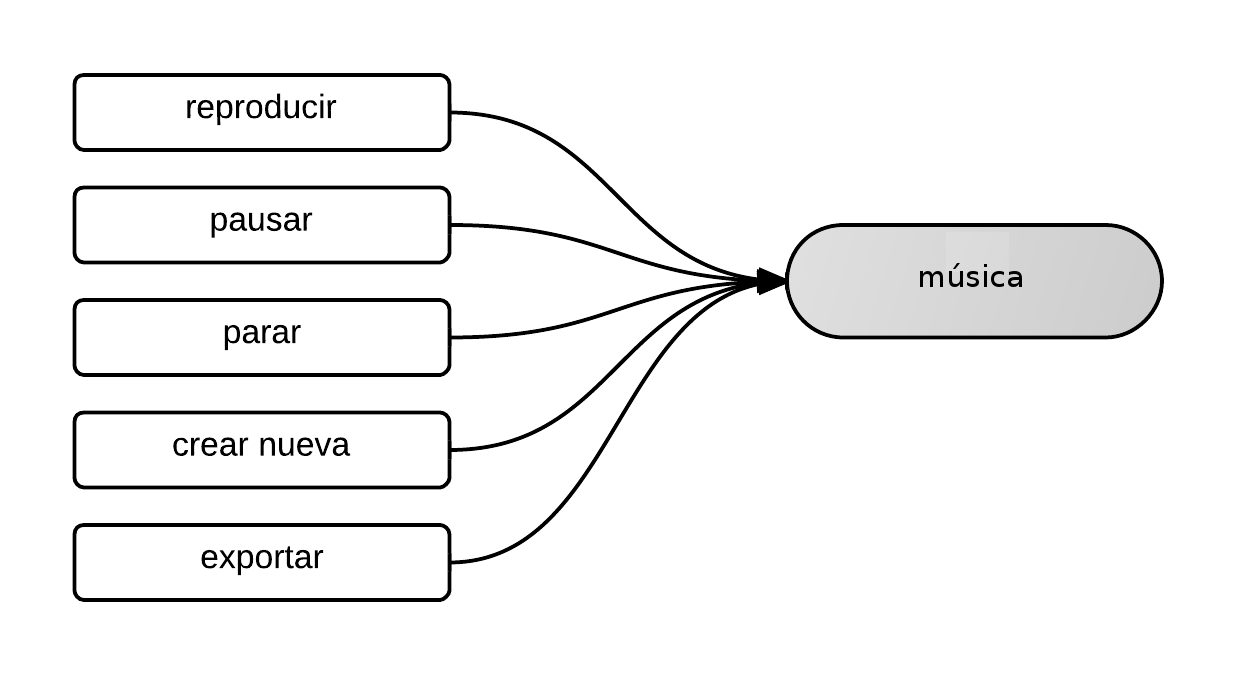
\includegraphics[width=0.5\textwidth]{./graphics/cmd-musica.png}
\caption{Comandos para reproducir, pausar, parar, exportar y crear una m\'usica}
\label{figure:cmd-crear-musica}
\end{figure}

\begin{figure}[ht]
\begin{minipage}[b]{0.5\linewidth}
\centering
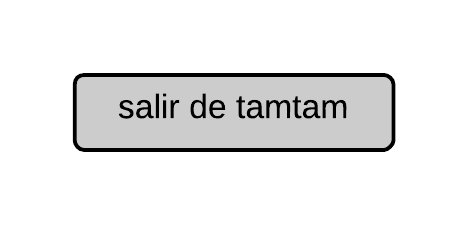
\includegraphics[width=0.6\linewidth]{./graphics/salir.png}
\caption{Comando para salir de la aplicaci\'on}
\label{figure:cmd-salir}
\end{minipage}
\quad
\begin{minipage}[b]{0.5\linewidth}
\centering
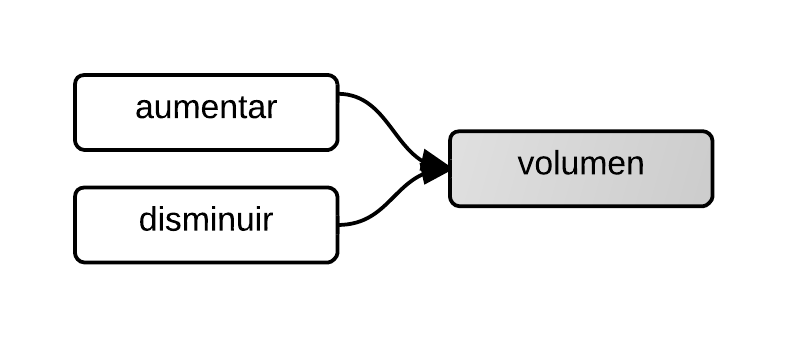
\includegraphics[width=0.6\linewidth]{./graphics/cmd-vol.png}
\caption{Comandos para aumentar/disminuir el volumen general}
\label{figure:cmd-vol}
\end{minipage}
\end{figure}


\begin{figure}[ht]
\begin{minipage}[b]{0.5\linewidth}
\centering
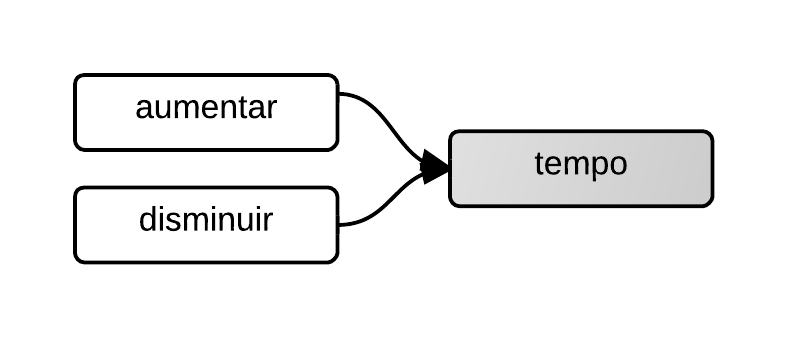
\includegraphics[width=0.6\linewidth]{./graphics/cmd-tempo.png}
\caption{Comandos para aumentar/disminuir el tempo general de al aplicaci\'on}
\label{figure:cmd-tempo}
\end{minipage}
\quad
\begin{minipage}[b]{0.5\linewidth}
\centering
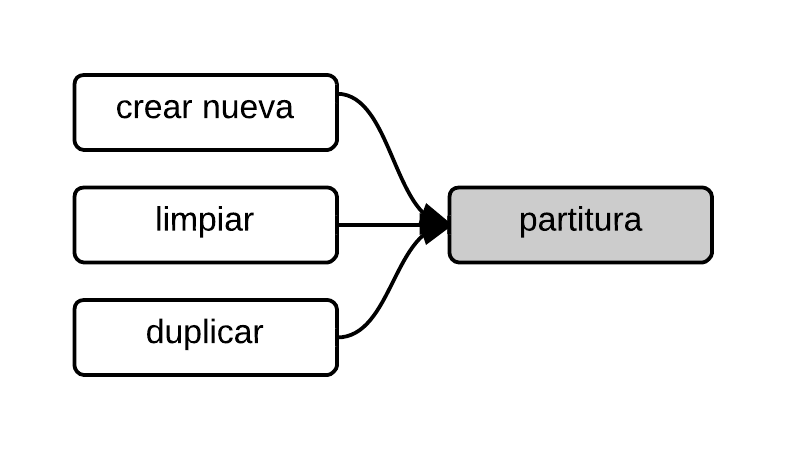
\includegraphics[width=0.6\linewidth]{./graphics/partitura-1.png}
\caption{Comandos para crear, limpiar y duplicar la partitura actual}
\label{figure:cmd-partitura-1}
\end{minipage}
\end{figure}


\begin{figure}[H]
\begin{minipage}[b]{0.5\linewidth}
\centering
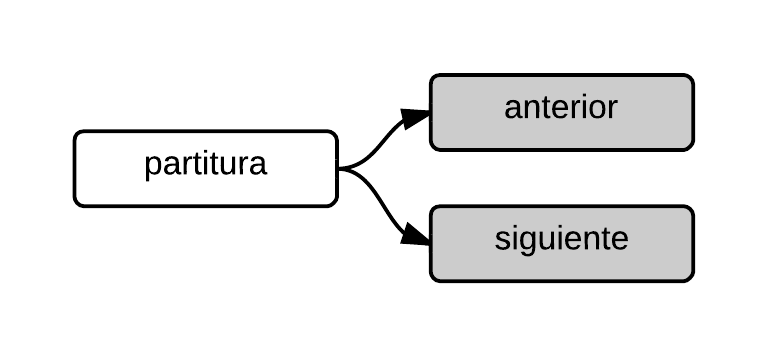
\includegraphics[width=0.6\linewidth]{./graphics/partitura-2.png}
\caption{Comandos para navegar entre partituras}
\label{figure:cmd-partitura-2}
\end{minipage}
\quad
\begin{minipage}[b]{0.5\linewidth}
\centering
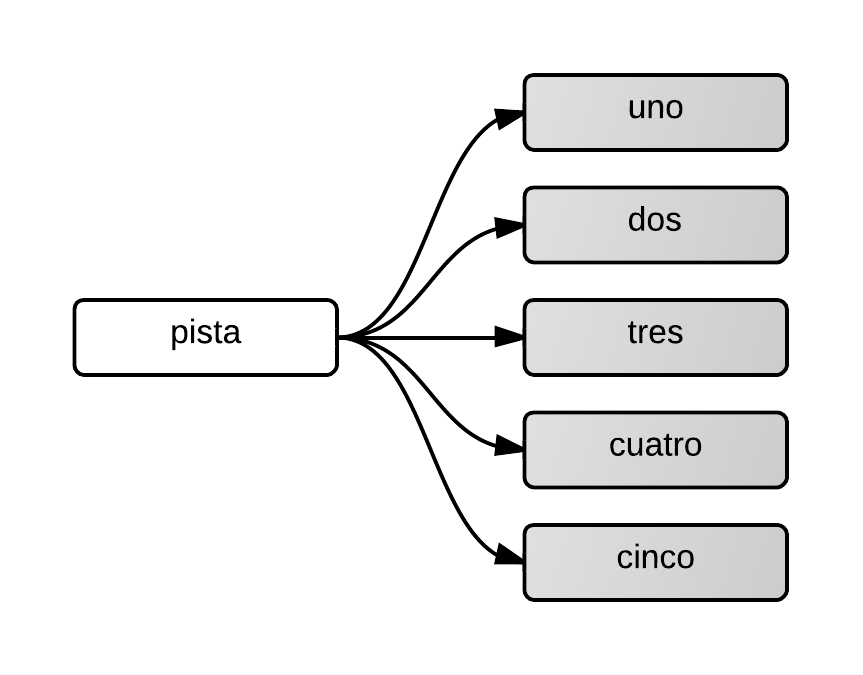
\includegraphics[width=0.6\linewidth]{./graphics/cmd-pista-1.png}
\caption{Comando para ubicarse en una pista}
\label{figure:cmd-partitura-1}
\end{minipage}
\end{figure}


\begin{figure}[H]
\begin{minipage}[b]{0.5\linewidth}
\centering
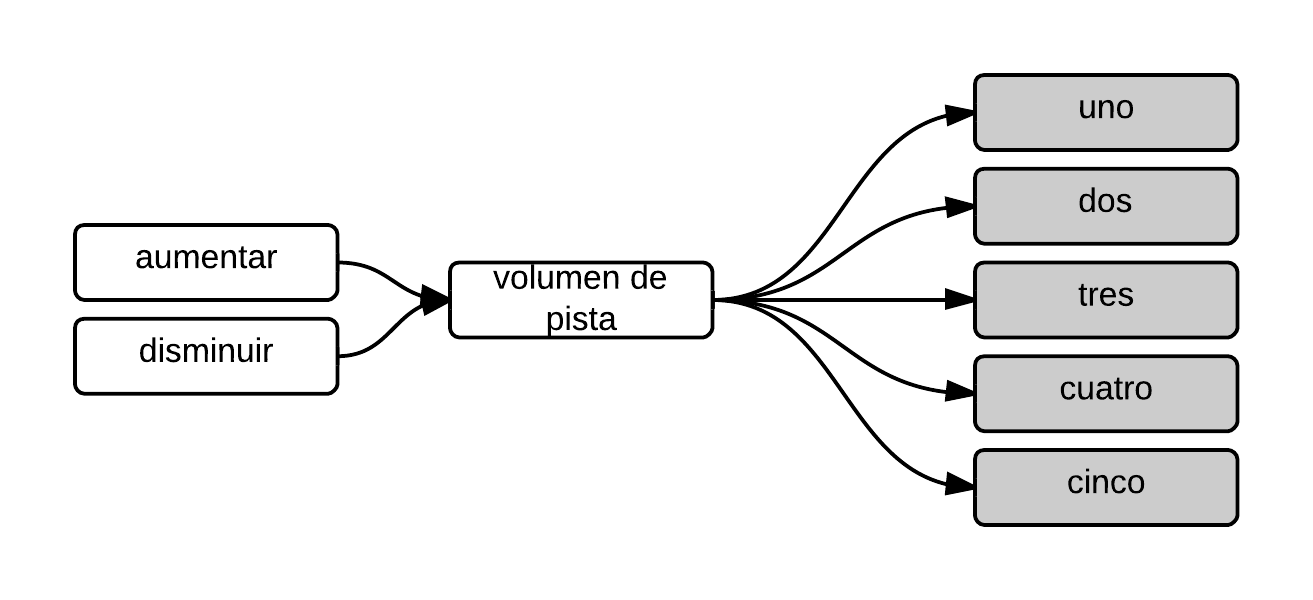
\includegraphics[width=0.8\linewidth]{./graphics/vol-pista.png}
\caption{Comandos para aumentar/disminuir el volumen de una pista en particular}
\label{figure:cmd-vol-pista}
\end{minipage}
\quad
\begin{minipage}[b]{0.5\linewidth}
\centering
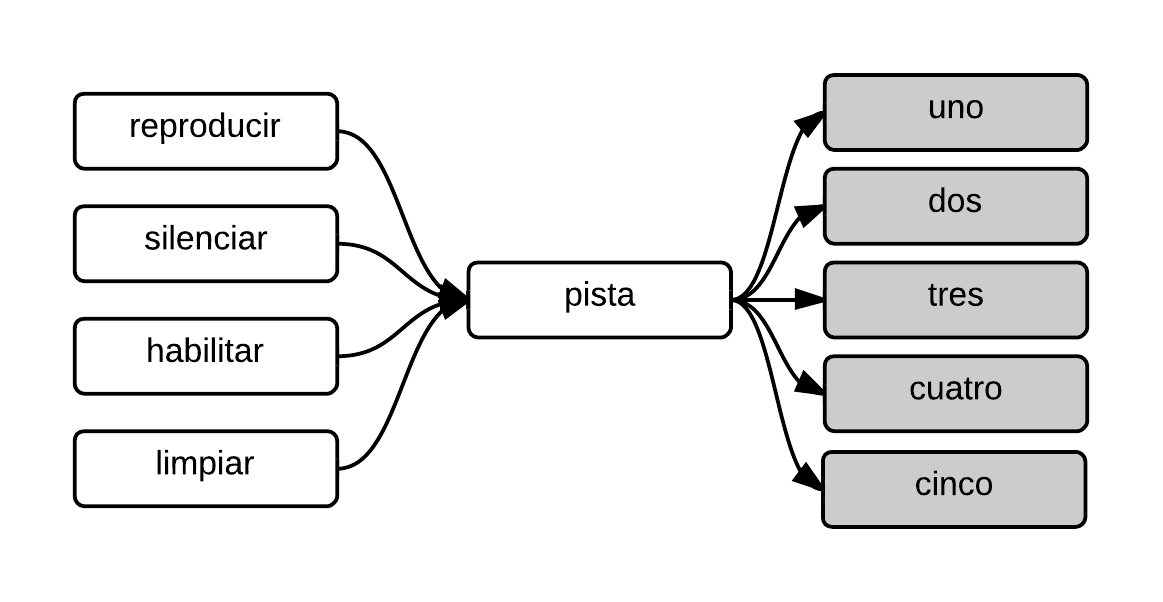
\includegraphics[width=0.9\linewidth]{./graphics/rep-pista.png}
\caption{Comandos para reproducir, silenciar, habilitar y limpiar una pista en particular}
\label{figure:cmd-rep-pista}
\end{minipage}
\end{figure}

\begin{figure}[H]
\centering
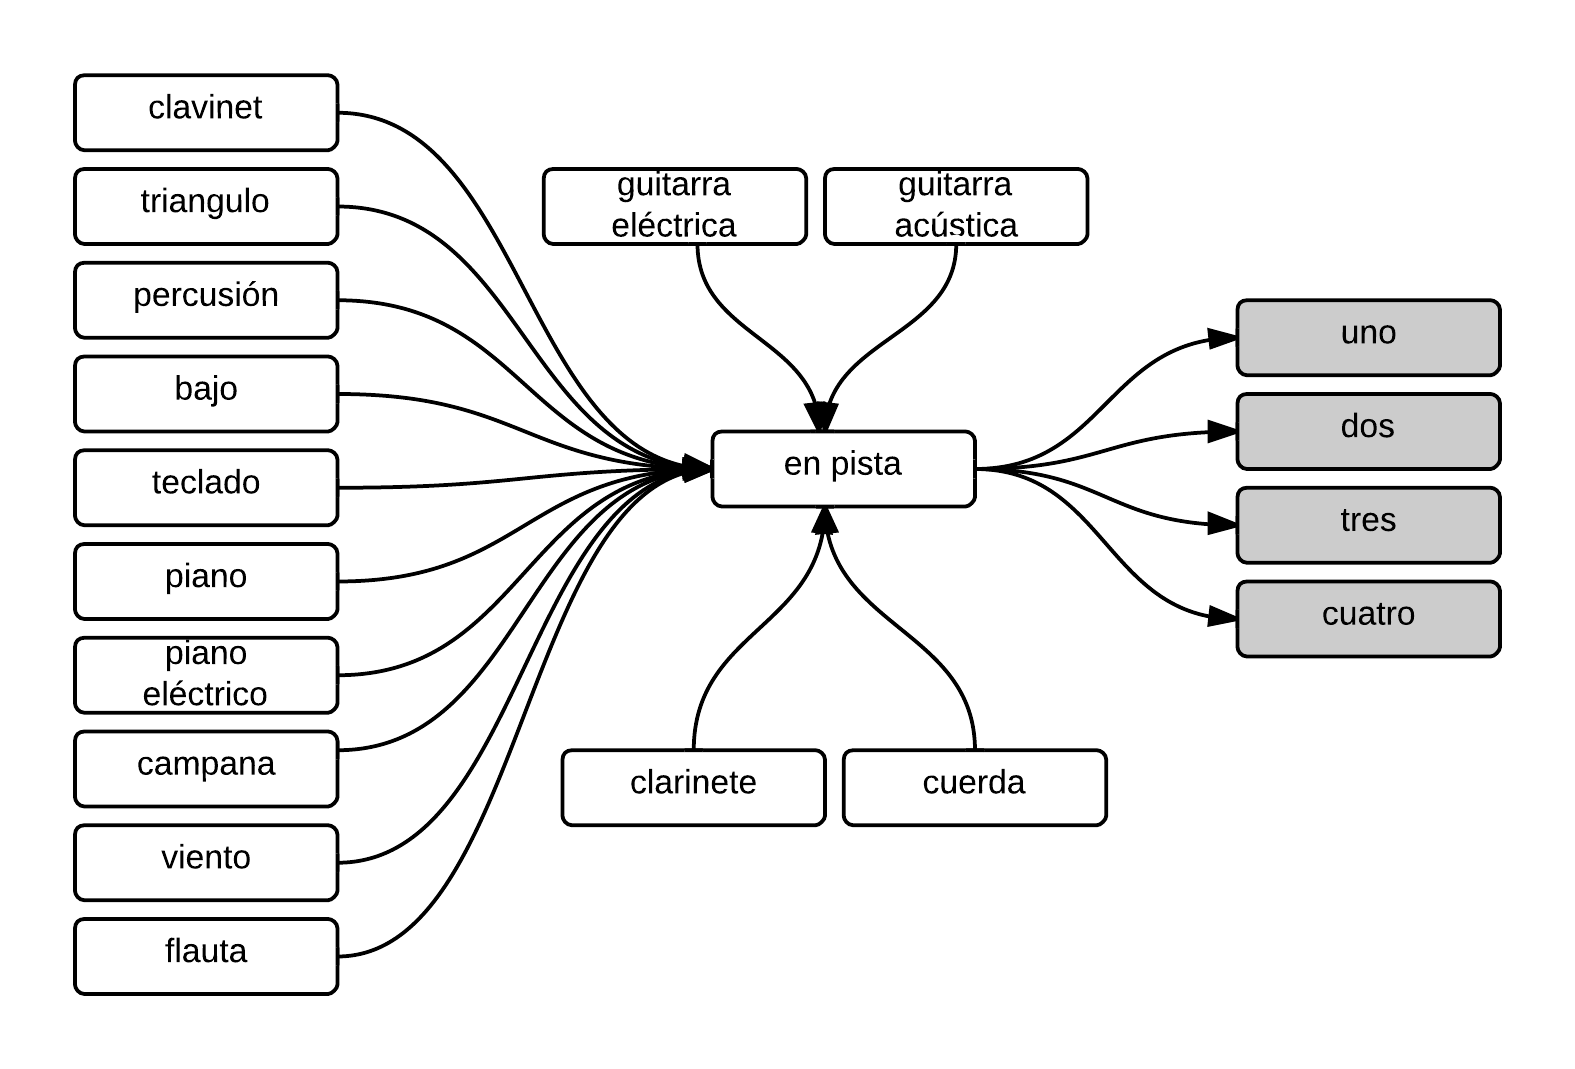
\includegraphics[width=0.8\textwidth]{./graphics/inst-p1-4.png}
\caption{Selecci\'on de instrumento para pistas del uno al cuatro}
\label{figure:cmd-inst-p1-4}
\end{figure}

\begin{figure}[H]
\begin{minipage}[b]{0.5\linewidth}
\centering
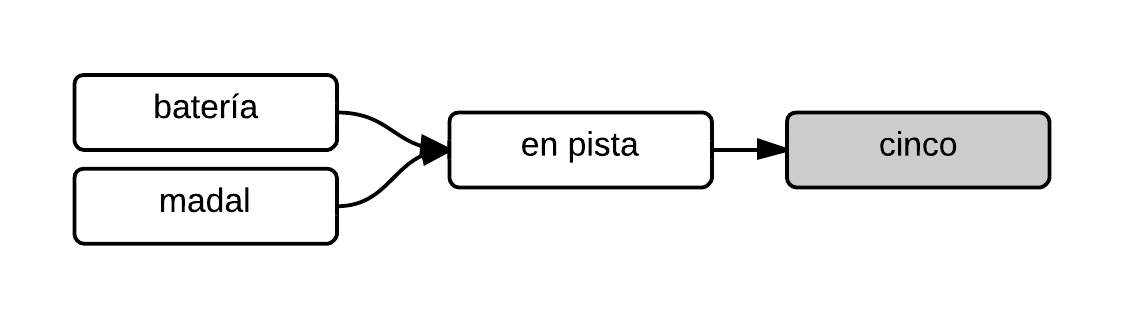
\includegraphics[width=1\linewidth]{./graphics/inst-p5.png}
\caption{Selecci\'on de instrumento para la pista cinco}
\label{figure:cmd-inst-p5}
\end{minipage}
\quad
\begin{minipage}[b]{0.5\linewidth}
\centering
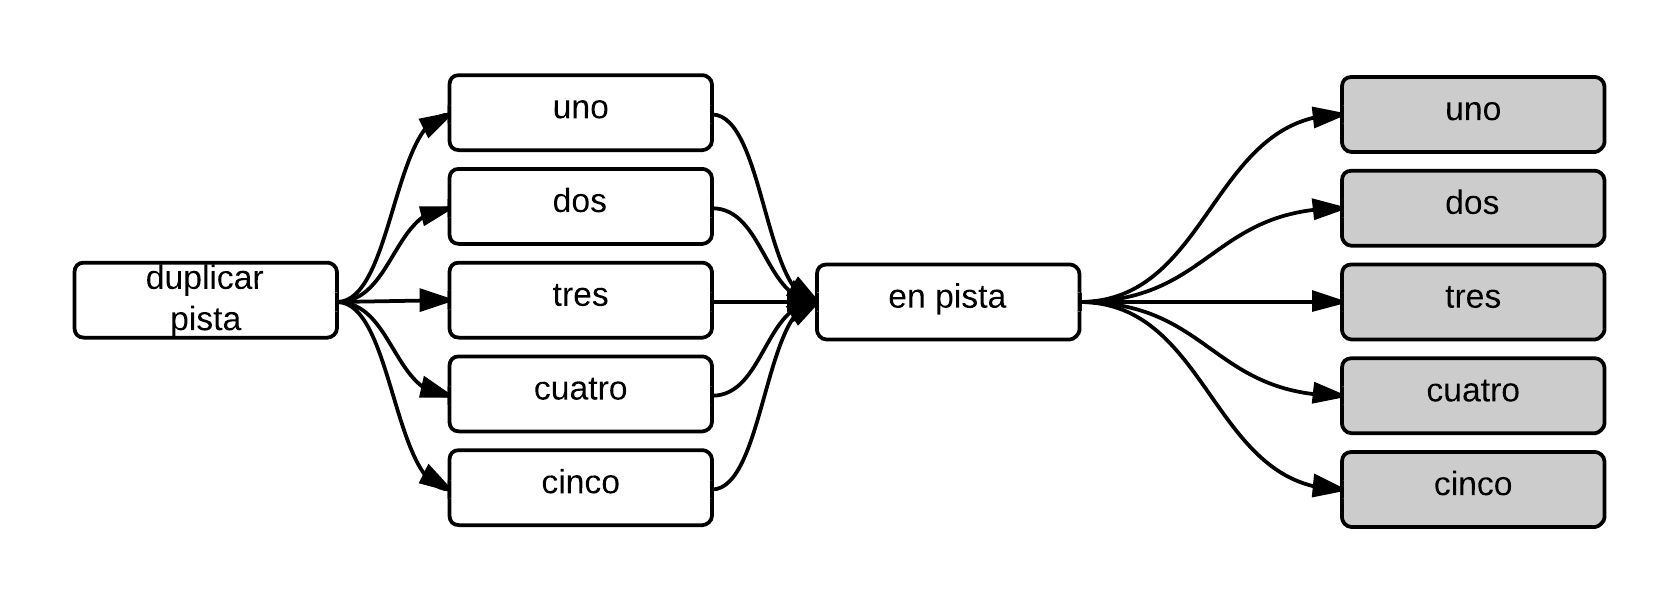
\includegraphics[width=1\linewidth]{./graphics/dup-pista.png}
\caption{Comando para duplicar las notas de una pista en otra}
\label{figure:cmd-dup-pista}
\end{minipage}
\end{figure}

\subsubsection{Comandos de Pista}

Este comando nos ubica dentro de una pista en particular. Por lo tanto, se debe
seleccionar una pista para poder utilizar este comando.

\begin{figure}[H]
\centering
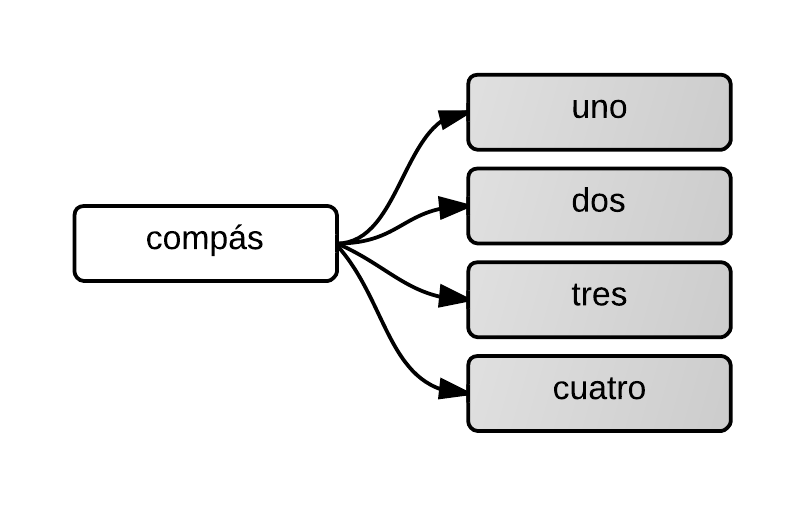
\includegraphics[width=0.4\linewidth]{./graphics/cmd-compas.png}
\caption{Comando para ubicarse en un comp\'as}
\label{figure:cmd-compas}
\quad
\end{figure}

\subsubsection{Comandos de Comp\'as}

Estos comandos son muy importantes para la aplicación ya que nos permiten crear, modificar, 
eliminar las notas musicales.

\begin{figure}[H]
\begin{minipage}[b]{0.5\linewidth}
\centering
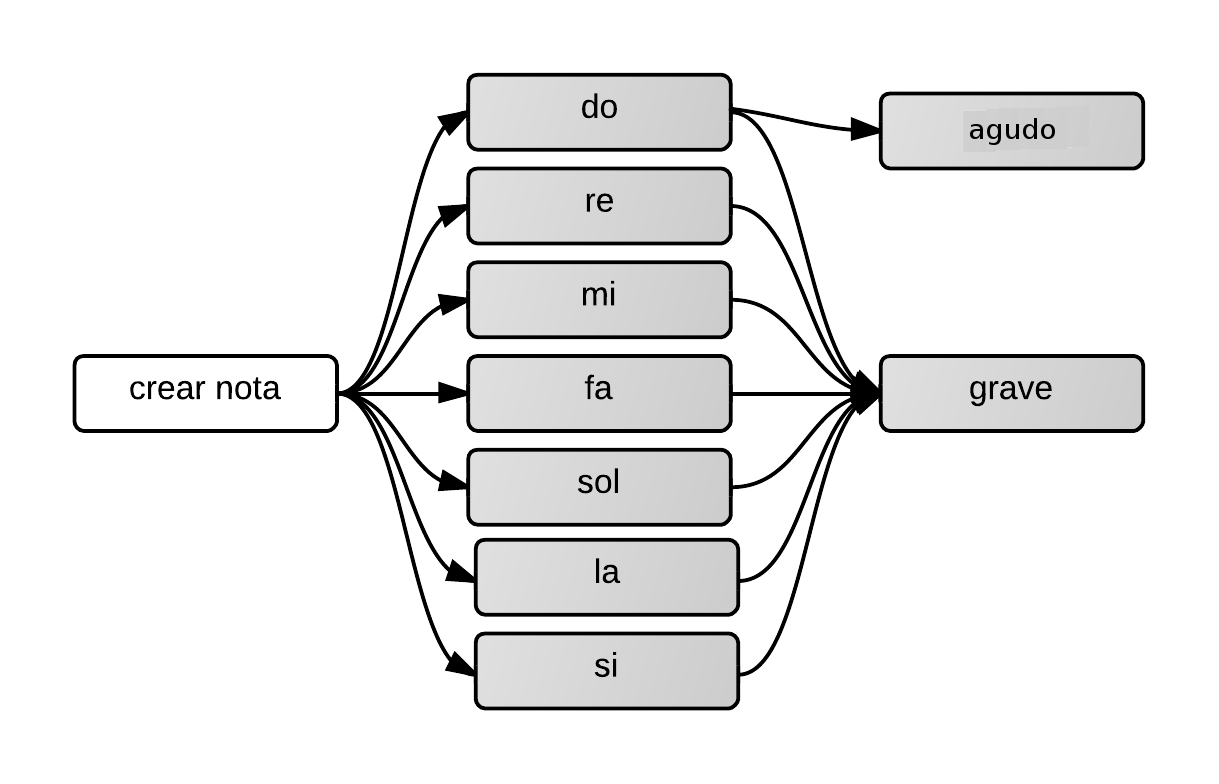
\includegraphics[width=1\linewidth]{./graphics/cmd-crear-nota.png}
\caption{Comando para crear una nota}
\label{figure:cmd-crear-nota}
\end{minipage}
\quad
\begin{minipage}[b]{0.5\linewidth}
\centering
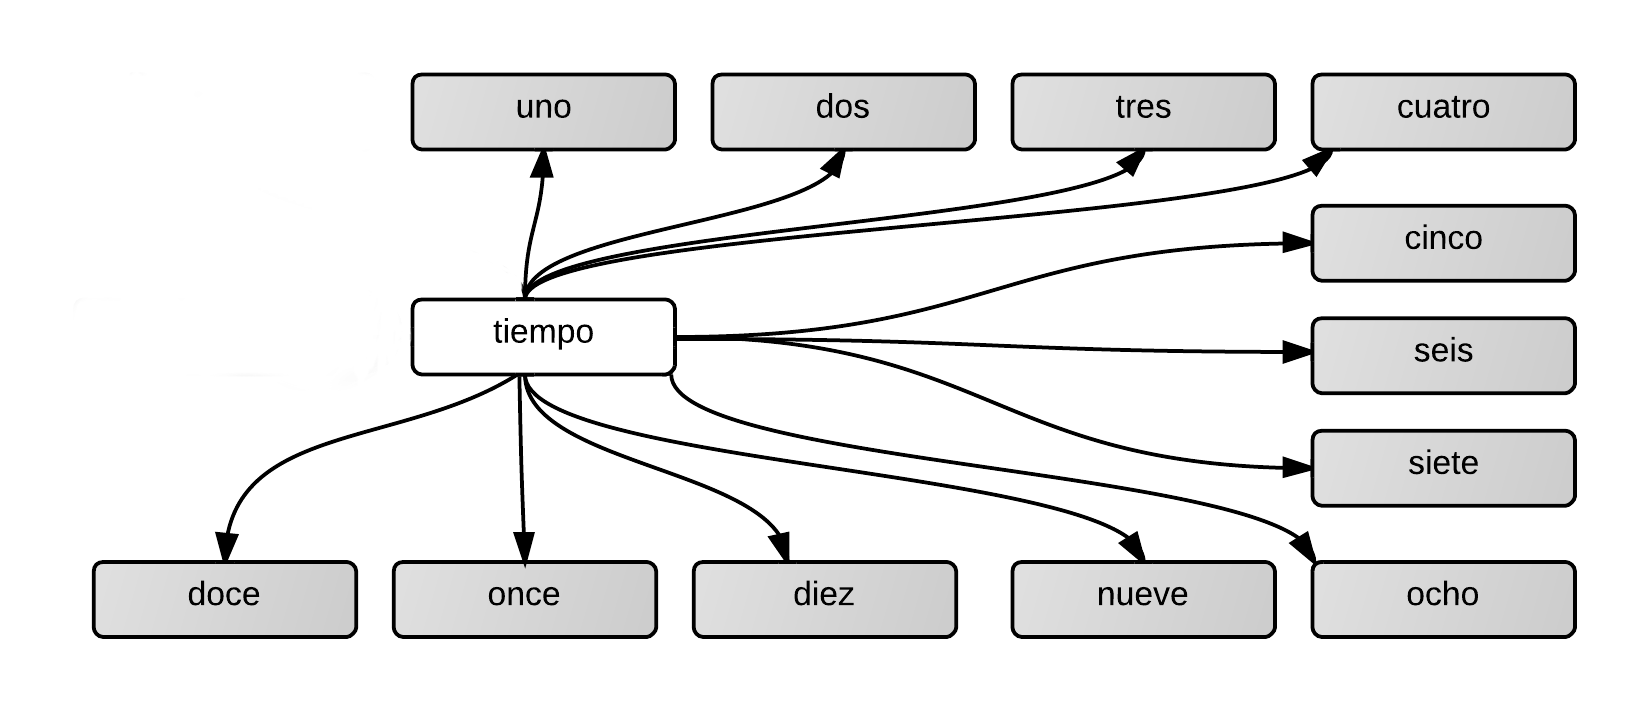
\includegraphics[width=1.1\linewidth]{./graphics/cmd-tiempo-compas.png}
\caption{Comando para ubicarse en un tiempo dado, dentro de un comp\'as}
\label{figure:cmd-tiempo-compas}
\end{minipage}
\end{figure}

\begin{figure}[H]
\begin{minipage}[b]{0.5\linewidth}
\centering
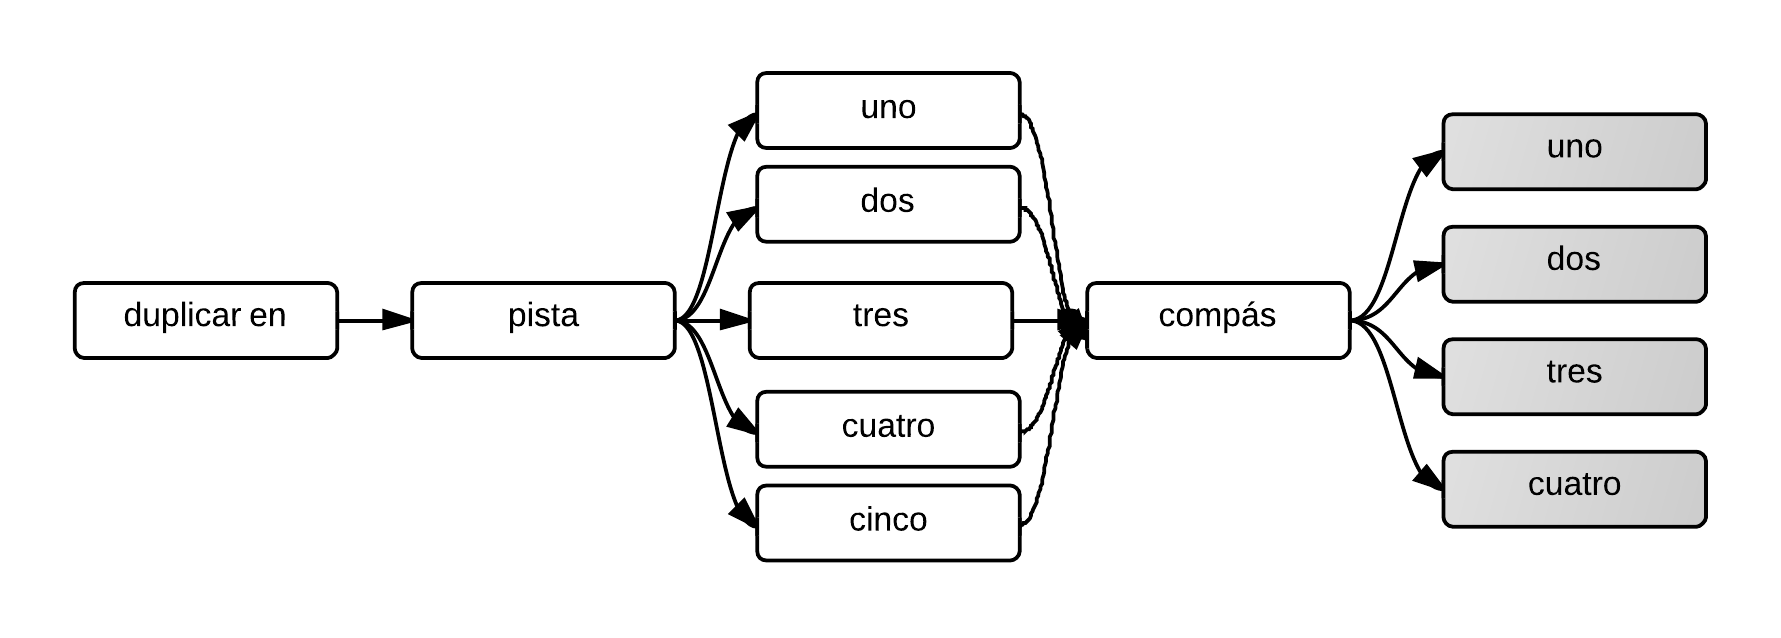
\includegraphics[width=1.2\linewidth]{./graphics/cmd-dup-nota.png}
\caption{Comando para duplicar una nota previamente seleccionada}
\label{figure:cmd-dup-nota}
\end{minipage}
\quad
\begin{minipage}[b]{0.5\linewidth}
\centering
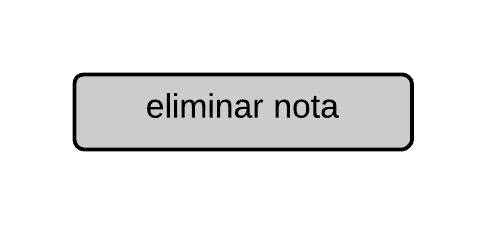
\includegraphics[width=0.5\linewidth]{./graphics/del-note.png}
\caption{Comando para eliminar un nota previamente seleccionada}
\label{figure:cmd-del-nota}
\end{minipage}
\end{figure}


\begin{figure}[H]
\begin{minipage}[b]{0.5\linewidth}
\centering
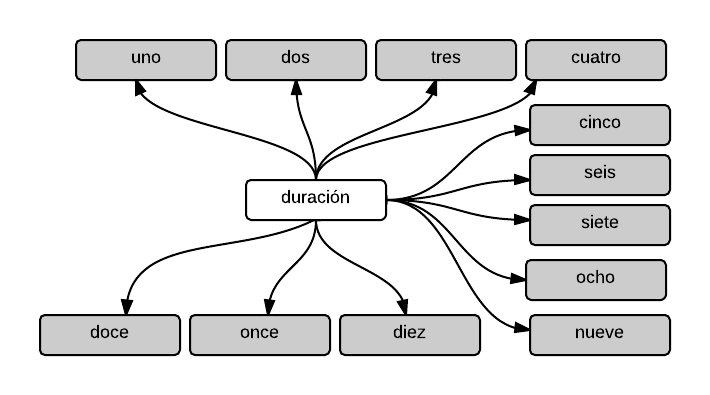
\includegraphics[width=0.9\linewidth]{./graphics/cmd-dur.png}
\caption{Comando que permite configurar la duraci\'on de una nota}
\label{figure:cmd-dur}
\end{minipage}
\quad
\begin{minipage}[b]{0.5\linewidth}
\centering
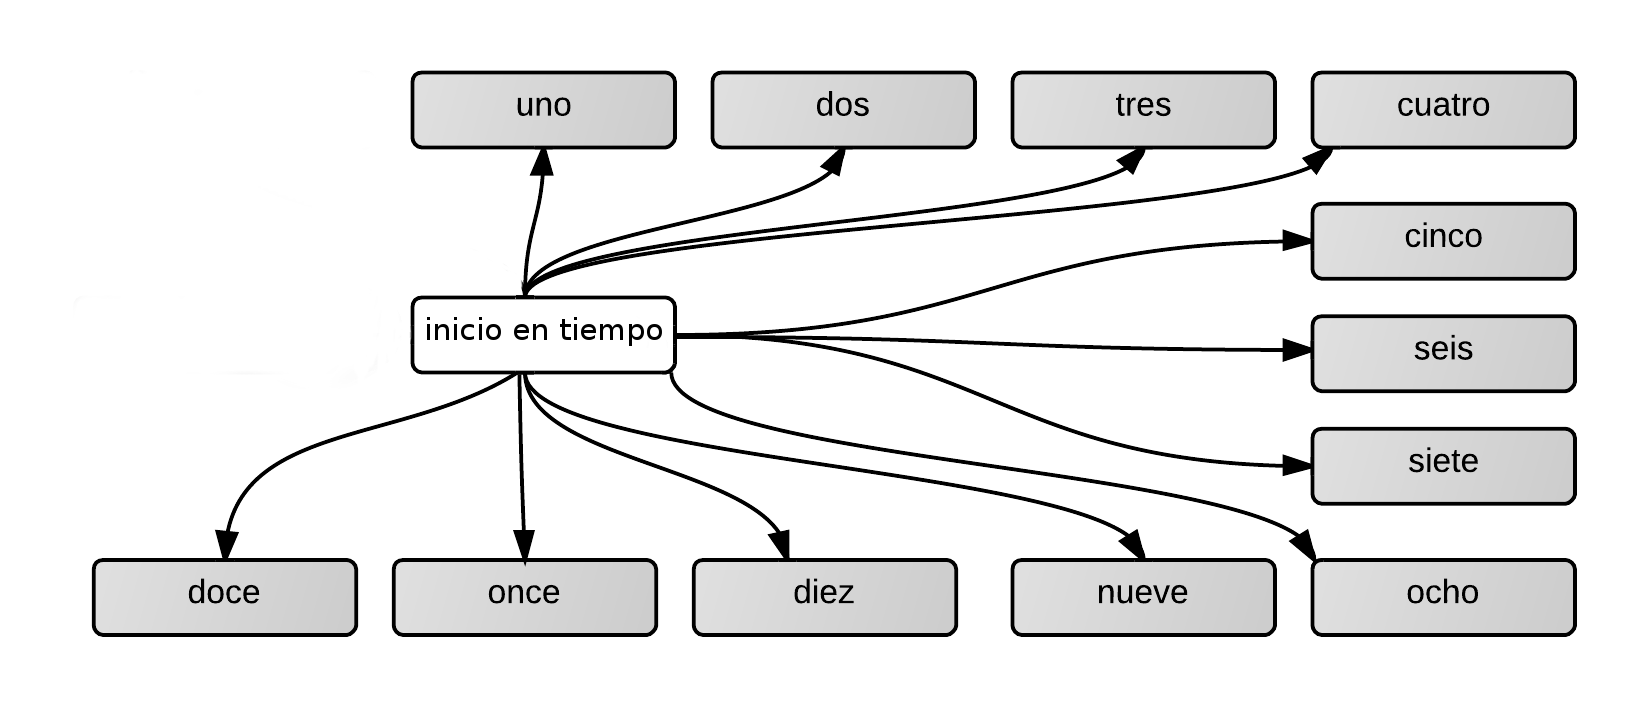
\includegraphics[width=1.1\linewidth]{./graphics/cmd-note-tiempo.png}
\caption{Comando que permite configurar el inicio de una nota dentro del comp\'as}
\label{figure:cmd-note-tiempo}
\end{minipage}
\end{figure}


\subsection{Diccionario}

Otro elemento requerido por \emph{Pocketsphinx} es el diccionario, que permite mapear
palabras a secuencia de fonemas. En la siguiente figura se muestra un fragmento del diccionario
utilizado por la aplicaci\'on.

\begin{figure}[H]
\begin{lstlisting}
REPRODUCIR RR E P R O D U S I R
PAUSAR P A U S A R
PARAR  P A R A R
GENERAR  J E N E R A R
PARTITURA P A R T I T U R A
SIGUIENTE S I G I E N T E
ANTERIOR A N T E R I O R
\end{lstlisting}
\caption{Fragmento del diccionario utilizad en \emph{Tamtam Listens}}
\end{figure}

La combinaci\'on de estos componentes es lo que permite a \emph{Pocketsphinx} realizar el
reconocimiento de los comandos de voz.
